\documentclass[10pt,landscape,a4paper]{article}
%\usepackage[utf8]{inputenc}
%\usepackage[ngerman]{babel}
\usepackage[normalem]{ulem}
\usepackage{tikz}
\usetikzlibrary{shapes,positioning,arrows,fit,calc,graphs,graphs.standard}
\usepackage[nosf]{kpfonts}
\usepackage[t1]{sourcesanspro}
%\usepackage[lf]{MyriadPro}
%\usepackage[lf,minionint]{MinionPro}
\usepackage{multicol}
\usepackage{wrapfig}
\usepackage[top=0mm,bottom=1mm,left=0mm,right=1mm]{geometry}
\usepackage[framemethod=tikz]{mdframed}
\usepackage{microtype}
%\usepackage{physics}
\usepackage{tabularx}
\usepackage{hhline}
\usepackage{makecell}
\usepackage{mathtools}
\usepackage{soul}

\usepackage{listings}

\DeclarePairedDelimiter{\ceil}{\lceil}{\rceil}

\newcommand\codeblue[1]{\textcolor{blue}{\code{#1}}}

\usepackage{lastpage}
\usepackage{datetime}
\yyyymmdddate
\renewcommand{\dateseparator}{-}
\let\bar\overline

\definecolor{myblue}{cmyk}{1,.72,0,.38}

\def\firstcircle{(0,0) circle (1.5cm)}
\def\secondcircle{(0:2cm) circle (1.5cm)}

\colorlet{circle edge}{myblue}
\colorlet{circle area}{myblue!5}

\tikzset{filled/.style={fill=circle area, draw=circle edge, thick},
outline/.style={draw=circle edge, thick}}

\pgfdeclarelayer{background}
\pgfsetlayers{background,main}

%\everymath\expandafter{\the\everymath \color{myblue}}
%\everydisplay\expandafter{\the\everydisplay \color{myblue}}


\renewcommand{\baselinestretch}{.8}
\pagestyle{empty}



\global\mdfdefinestyle{header}{%
  linecolor=gray,linewidth=1pt,%
  leftmargin=0mm,rightmargin=0mm,skipbelow=0mm,skipabove=0mm,
}

\newcommand{\header}{
  \begin{mdframed}[style=header]
    \footnotesize
    \sffamily
    ACC1701XA Midterms Cheatsheet v1.1 (\today)\\
    by~Your Name,~page~\thepage~of~\pageref{LastPage}
  \end{mdframed}
}

% Custom command for keywords
\definecolor{highlight}{RGB}{251,243,218}
\newcommand{\keyword}[2][]{\sethlcolor{highlight}\hl{\textbf{#2}} #1 - }
\newcommand{\ilkeyword}[1]{\sethlcolor{highlight}\hl{\textbf{#1}}}

\let\counterwithout\relax
\let\counterwithin\relax
\usepackage{chngcntr}

\usepackage{verbatim}

\usepackage{etoolbox}
\makeatletter
\preto{\@verbatim}{\topsep=0pt \partopsep=0pt }
\makeatother

\counterwithin*{equation}{section}
\counterwithin*{equation}{subsection}
\usepackage{enumitem}
\newlist{legal}{enumerate}{10}
\setlist[legal]{label*=\arabic*.,leftmargin=2.5mm}
\setlist[itemize]{leftmargin=3mm}
\setlist[enumerate]{leftmargin=3.5mm}
\setlist{nosep}
\usepackage{minted}

\def\code#1{\texttt{#1}}

\newenvironment{descitemize} % a mixture of description and itemize
{\begin{description}[leftmargin=*,before=\let\makelabel\descitemlabel]}
{\end{description}}

\newcommand{\descitemlabel}[1]{%
  \textbullet\ \textbf{#1}%
}
\makeatletter



\renewcommand{\section}{\@startsection{section}{1}{0mm}%
  {.2ex}%
  {.2ex}%x
{\color{myblue}\sffamily\small\bfseries}}
\renewcommand{\subsection}{\@startsection{subsection}{1}{0mm}%
  {.2ex}%
  {.2ex}%x
{\sffamily\bfseries}}
\renewcommand{\subsubsection}{\@startsection{subsubsection}{1}{0mm}%
  {.2ex}%
  {.2ex}%x
{\rmfamily\bfseries}}

\global\let\tikz@ensure@dollar@catcode=\relax

\def\mathcolor#1#{\@mathcolor{#1}}
\def\@mathcolor#1#2#3{%
  \protect\leavevmode
  \begingroup
  \color#1{#2}#3%
  \endgroup
}

\makeatother
\setlength{\parindent}{0pt}

\setminted{tabsize=2, breaklines}
% Remove belowskip of minted
\setlength\partopsep{-\topsep}

\newcolumntype{a}{>{\hsize=1.5\hsize}X}
% \newcolumntype{b}{>{\hsize=.25\hsize}X}

\setlength\columnsep{1.5pt}
\setlength\columnseprule{0.1pt}

\begin{document}
\setlength{\abovedisplayskip}{0pt}
\setlength{\belowdisplayskip}{0pt}

% \header

\scriptsize
\begin{multicols*}{4}
  % \raggedcolumns

  % \section{Heading 1}
  % \begin{itemize}
  %   \item Point 1
  %   \item Point 2
  % \end{itemize}

  % \subsection{Heading 1.1}
  % \begin{itemize}
  %   \item Point A
  %   \item Point B
  % \end{itemize}

  % \subsubsection{Heading 1.1.1}
  % \begin{itemize}
  %   \item Point X
  %   \item Point Y
  % \end{itemize}

  % \begin{tabular}{l}
  %   \includegraphics[width=0.5\linewidth]{placeholder-image}
  % \end{tabular}
  % \begin{minipage}{0.15\columnwidth}
  %   Placeholder note for image
  % \end{minipage}

  % \begin{minipage}{0.5\columnwidth}
  %   \begin{tabularx}{\linewidth}{X}
  %     Left Column Text Placeholder abcdefg
  %   \end{tabularx}
  % \end{minipage}
  % \hfill
  % \begin{minipage}{0.5\columnwidth}
  %   \begin{tabularx}{\linewidth}{X}
  %     Right Column Text Placeholder hijklmnop
  %   \end{tabularx}
  % \end{minipage}

  % \begin{minted}{C}
  % // comment for codeblock
  % int main() {
  %   return 0;
  % }
  % \end{minted}

%   % Title box
% \begin{center}
%     \fbox{
%         \parbox{0.8\linewidth}{
%             \centering \textcolor{black}{
%                 {\Large\textbf{CS2109S}} \\
%                 \normalsize{AY22/23 Sem 2}} \\
%                 {\footnotesize \textcolor{gray}{github.com/jasonqiu212}}
%         }
%     }
% \end{center}

\section{01. Introduction}

\begin{itemize}
    \item \keyword{Agent}{Anything that can perceive its environment through sensors and acting upon that env. through actuators}
    \item \keyword{Agent Function}{Maps from percept histories to actions}
    \item \keyword{Rational Agent}{Chooses an action that is expected to maximize its performance measure, given by percept sequence and built-in knowledge}
    \item \keyword{Autonomous Agent}{If behavior is determined by its own expereince}
\end{itemize}

\subsection{Performance Measure of Function}

\begin{itemize}
    \item Motivation: For an agent to do the right thing, need a measure of goodness
\end{itemize}

\subsection{Defining the Problem: PEAS}

\begin{enumerate}
    \item Performance measure
    \item Environment
    \item Actuators
    \item Sensors
\end{enumerate}

\subsection{Characterizing the Environment}

\begin{enumerate}
    \item \keyword{Fully observable}{(vs. Partially) Agent's sensors can access complete state of env. all the time}
    \item \keyword{Deterministic}{(vs. Stochastic) Next state of env. is determined by \textbf{current state} and \textbf{action executed by agent}}
    \begin{itemize}
        \item \keyword{Strategic}{If env. is deterministic except for actions of other agents}
    \end{itemize}
    \item \keyword{Episodic}{(vs. Sequential) Agent's experience is divided into atomic \textbf{episodes}, where each episode includes perceiving and an action, and \textbf{action depends on episode} itself}
    \item \keyword{Static}{(vs. Dynamic) Env. is unchanged while agent is deciding}
    \begin{itemize}
        \item \keyword{Semi}{Time does not affect env., but affects performance score}
    \end{itemize}
    \item \keyword{Discrete}{(vs. Continuous) Discrete num. of percepts and actions}
    \item \keyword{Single Agent}{(vs. Multi-agent) Agent operating by itself in an env.}
\end{enumerate}

\subsection{Implementing Agents (in ascending complexity)}

\begin{enumerate}
    \item \keyword{Simple Reflex Agents}{Fixed conditional rules}
    \item \keyword{Model-based Reflex Agents}{Stores percept history to make decisions about internal model of world with conditional rules. Eg. Roomba}
    \item \keyword{Goal-based Agents}{Keep in mind a goal and action aims to achieve it}
    \item \keyword{Utility-based Agents}{Find best way to achieve goal}
    \item \keyword{Learning Agents}{Learn from previous experiences}
\end{enumerate}

\subsection{Exploitation vs. Exploration}

\begin{itemize}
    \item \keyword{Exploitation}{Maximize expected utility using current knowledge of world}
    \item \keyword{Exploration}{Learn more about the world to improve future gains. May not always maximize performance measure.}
\end{itemize}

\section{02. Uninformed Search}

\begin{itemize}
    \item Deterministic, fully observable
    \item \keyword{Tree Search}{Can revisit nodes}
    \item \keyword{Graph Search}{Tracks visited (Tree Search + Memoization)}
    \item \keyword{Uninformed Search}{Uses only information available in problem definition}
\end{itemize}

\subsection{Formulating the Problem}

\begin{enumerate}
    \item How to represent state in problem?
    \item Initial state
    \item Actions: Successor function
    \item Goal test
    \item Path cost
\end{enumerate}

\begin{itemize}
    \item \keyword{Abstraction Function}{Maps abstracted representation to real world state}
    \item \keyword{Representation Invariant}{$I(c) = \textbf{True} \rightarrow \exists a \textbf{ s.t. } AF(c) = a$}
\end{itemize}

\subsection{Breadth-first Search}

\begin{itemize}
    \item Idea: Expand shallowest unexpanded node using \textbf{queue}
    \item Given: $b$: Branching factor and $d$: Depth of optimal solution
    \item Complete: Yes (if tree is finite)
    \item Time: $O(b^d)$
    \item Space: $O(b^d)$
    \item Optimal: Yes (if cost = 1)
    \item BFS is Uniform-cost Search with same cost
\end{itemize}

\subsection{Uniform-cost Search}

\begin{itemize}
    \item Idea: Expand least-cost unexpanded node using \textbf{priority queue} (Dijkstra's)
    \item Given: $C^*$: Cost of optimal solution
    \item Complete: Yes (if step cost $\geq \epsilon$ where $\epsilon \geq 0$)
    \item Time: $O(b^{(C^* / \epsilon)})$ ($C^* / \epsilon$ is approx. number of layers)
    \item Space: $O(b^{(C^* / \epsilon)})$
    \item Optimal: Yes
\end{itemize}

\subsection{Depth-first Search}

\begin{itemize}
    \item Idea: Expand deepest unexpanded node using \textbf{stack}
    \item Given: $m$: Maximum depth of tree
    \item Complete: No (fails with infinite depth or loops)
    \item Time: $O(b^m)$
    \item Space: $O(bm)$ (better than BFS)
    \item Optimal: No
\end{itemize}

\subsection{Depth-limited Search}

\begin{itemize}
    \item Motivation: How to handle infinite depth for DFS?
    \item Idea: DFS with depth limit $I$ where nodes at depth $I$ have no children
    \item Time: $b^0 + b^1 + ... + b^{(d - 1)} + b^d = O(b^d)$
\end{itemize}

\subsection{Iterative Deepening Search}

\begin{itemize}
    \item Motivation: How to determine depth limit? We don't.
    \item Idea: Try different depths for depth-limited search
    \begin{itemize}
        \item BFS pretending to be DFS to save space
    \end{itemize}
    \item Complete: Yes
    \item Time: $(d + 1)b^0 + db^1 + ... + b^d = O(b^d)$ (More overhead than DLS)
    \item Space: $O(bd)$
\end{itemize}

\subsection{Summary}

\begin{tabular}{ |c|c|c|c|c|c| }
    \hline
    & \textbf{BFS} & \textbf{Uniform Cost} & \textbf{DFS} & \textbf{DLS} & \textbf{IDS} \\
    \hline
    \textbf{Complete} & Yes & Yes & No & No & Yes \\
    \hline
    \textbf{Time} & $O(b^d)$ & $O(b^{C^* / \epsilon})$ & $O(b^m)$ & $O(b^l)$ & $O(b^d)$ \\
    \hline
    \textbf{Space} & $O(b^d)$ & $O(b^{C^* / \epsilon})$ & $O(bm)$ & $O(bl)$ & $O(bd)$ \\
    \hline
    \textbf{Optimal} & Yes & Yes & No & No & No \\
    \hline
\end{tabular}

\subsection{Bidirectional Search}

\begin{itemize}
    \item Idea: Search both forwards from initial state and backwards from goal state. Stop when searches meet.
    \item Time: $O(2 b^{d/2})$
    \item Operators must be reversible
    \item Can have many goal states
    \item How to check if node intersects with other half?
\end{itemize}

\section{03. Informed Search}

\subsection{Heuristic}

\begin{itemize}
    \item \keyword{Heuristic}{Estimated cost from $n$ to goal}
    \item \keyword{Admissible}{$h(n)$ is admissible if, for every node $n$, $h(n) \leq h^*(n)$ where $h^*$ is the true cost}
    \begin{itemize}
        \item if $h$ is admissible, then A* using tree search is optimal
    \end{itemize}
    \item \keyword{Consistent}{$h(n)$ is consistent if, for every node $n$ and every successor $n'$ of $n$ generated by action $a$, $h(n) \leq c(n, a, n') + h(n')$}
    \begin{itemize}
        \item Triangle inequality
        \item If $h$ is consistent, $f(n)$ is non-decreasing along any path ($f(n') \geq f(n)$)
        \item If $h$ is consistent, then $h$ is admissible
        \item if $h$ is admissible, then A* using graph search is optimal
    \end{itemize}
\end{itemize}

\subsubsection{Dominance}

\begin{itemize}
    \item If $h_2 (n) \geq h_1 (n)$ for all $n$, then $h_2$ \ilkeyword{dominates} $h_1$
    \item If $h_2$ \ilkeyword{dominates} $h_1$ and both are admissible, then $h_2$ is better for search
\end{itemize}

\subsubsection{How to invent admissible heuristic?}

\begin{itemize}
    \item Set fewer restrictions on actions
    \item E.g. Number of misplaced tiles, Total manhattan distance
\end{itemize}

\subsection{Best-first Search}

\begin{itemize}
    \item Idea: Expand most desirable node using priority queue
    \item Evaluation Function: $f(n) = h(n)$
    \item Complete: No. Possible to be stuck in loop
    \item Time and space: $O(b^m)$
    \item Optimal: No
\end{itemize}

\subsection{A* Search}

\begin{itemize}
    \item Idea: Take note of cost so far and heuristic
    \item Evaluation Function: $f(n) = g(n) + h(n)$ where $g(n)$ is cost to reach $n$ 
    \item Complete: Yes, unless non-increasing, since cost is factored in
    \item Time and space: Same as BFS
    \item Optimal: Yes, depending on the heuristic
\end{itemize}

\subsection{Iterative Deepening A* Search (IDA*)}

\begin{itemize}
    \item Motivation: How can we save space?
    \item Idea: Have a cutoff for $f$ and remember the best $f$ that exceeds cutoff
    \begin{itemize}
        \item Similar to IDS. Linear space complexity.
    \end{itemize}
    \item Optimal and complete
\end{itemize}

\subsection{Simplified Memory A* Search (SMA*)}

\begin{itemize}
    \item Motivation: How can we save space?
    \item Idea: Do normal A*. If memory is full, drop node with worst $f$.
    \item Lose completeness
\end{itemize}

\subsection{Local Search}

\begin{itemize}
    \item Motivation: What if the goal state is the solution? The path is irrelevant.
    \item Idea: Keep single current state and try improving it
    \item Formulating the problem:
    \begin{enumerate}
        \item Initial state
        \item Actions: Successor function
        \item Good heuristic
        \item Goal test
    \end{enumerate}
\end{itemize}

\subsubsection{Hill-climbing}

\begin{itemize}
    \item Idea: Generate successors from current and pick the best using heuristic
    \item What if stuck into local minima?
    \begin{itemize}
        \item Introduce randomness
        \item \keyword{Simulated Annealing Search}{Allow some bad moves and gradually decrease frequency}
    \end{itemize}
    \item Why only keep 1 best state?
    \begin{itemize}
        \item \keyword{Beam Search}{Perform $k$ hill-climbing searches in parallel}
    \end{itemize}
    \item How to generate successors?
    \begin{itemize}
        \item \keyword{Genetic Algorithms}{Successsor is generated by combining 2 parent states}
    \end{itemize}
\end{itemize}

\section{04. Adversarial Search}

\begin{itemize}
    \item Assumption: Opponents reacts rationally
    \item Formulating the problem:
    \begin{itemize}
        \item Initial state
        \item Successor function
        \item Terminal test
        \item Utility function: Measures how good the move is for a player
    \end{itemize}
\end{itemize}

\subsection{Minimax}

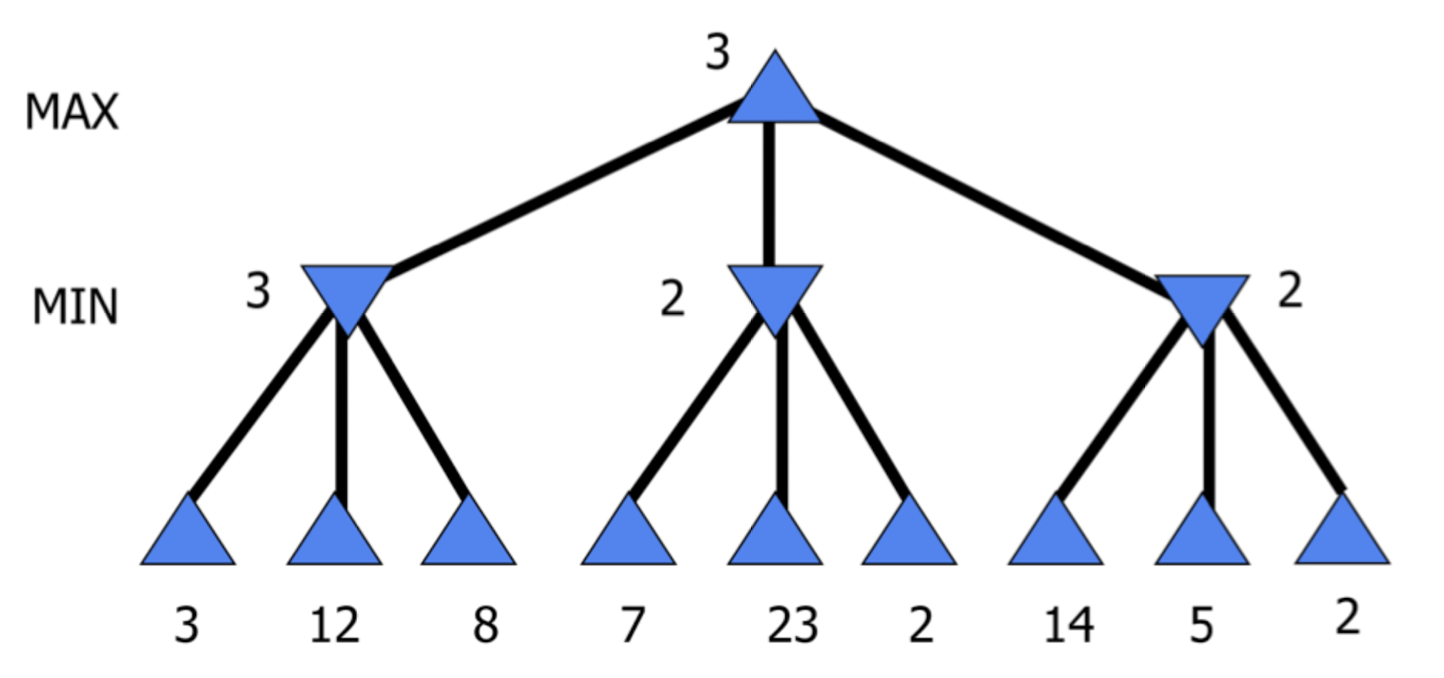
\includegraphics[scale=0.2]{minimax}

\begin{itemize}
    \item Idea: Choose move that yields highest minimax value using DFS
    \item Complete: Yes (if tree is finite)
    \item Time: $O(b^m)$
    \item Space: $O(bm)$
    \item Optimal: Yes (against an optimal opponent)
\end{itemize}

\subsubsection{How to Draw a Game Tree?}

\begin{itemize}
    \item Do not have repeated states \textbf{per level}
\end{itemize}

\subsection{Alpha-Beta Pruning}

\begin{itemize}
    \item Motivation: How to save time for Minimax?
    \item Idea: By tracking max. and min. values so far, can prune some paths that we would never choose
    \begin{enumerate}
        \item $\alpha$ contains max. and $\beta$ contains min.
        \item Initially, $\alpha = -\infty$ and $\beta = \infty$
        \item When going down, copy $\alpha$ and $\beta$
        \item Prune if $\alpha \geq \beta$
        \item When going up, depending on MIN/MAX level, update $\alpha$ or $\beta$
    \end{enumerate}
    \item With perfect ordering, time complexity: $O(b^{m/2})$. Doubles search depth.
\end{itemize}

\subsection{Resource Limits}

\begin{itemize}
    \item In reality, search space for games can be very large. $\alpha$-$\beta$ pruning also not fast enough.
    \item Solution: Limit depth (Only see a finite moves ahead) and determine best move using evaluation function to estimate desirability of position (Heuristic)
    \item Other hacks:
    \begin{itemize}
        \item \keyword{Transpoisitions}{Memoize equivalent states}
        \item Pre-computation of opening/closing moves
    \end{itemize}
\end{itemize}

\section{05. Introduction to Machine Learning}

\begin{itemize}
    \item A machine learns if it improves performance P on task T based on experience E. Where T must be fixed, P must be measurable, E must exist
\end{itemize}

\subsubsection{Types of Feedback}

\begin{itemize}
    \item \keyword{Supervised}{Correct answer given for each example}
    \begin{itemize}
        \item \keyword{Regression}{Predict results within continuous output}
        \item \keyword{Classification}{Predict results in discrete output}
    \end{itemize}
    \item \keyword{Unsupervised}{No answers given}
    \item \keyword{Weakly supervised}{Answer given, but not precise}
    \item \keyword{Reinforcement}{Occasional rewards given}
\end{itemize}

\subsection{Decision Trees}

\begin{itemize}
    \item DT can express any function of input attributes, if data is consistent
    \item Goal: Make DT \textbf{compact}. How?
\end{itemize}

\subsubsection{Information Theory}

\begin{itemize}
    \item Idea: Choose attribute that splits examples into subsets that are ideally 'all positive' or 'all negative'
    \item \keyword{Entropy}{Measure of randomness in set of data}
\end{itemize}

\[I(P(v_1), ..., P(v_n)) = - \sum^{n}_{i = 1} P(v_i) \log_{2} P(v_i)\]

\begin{itemize}
    \item For data with $p$ positive examples and $n$ negative examples:
\end{itemize}

\begin{multicols*}{2}
    
    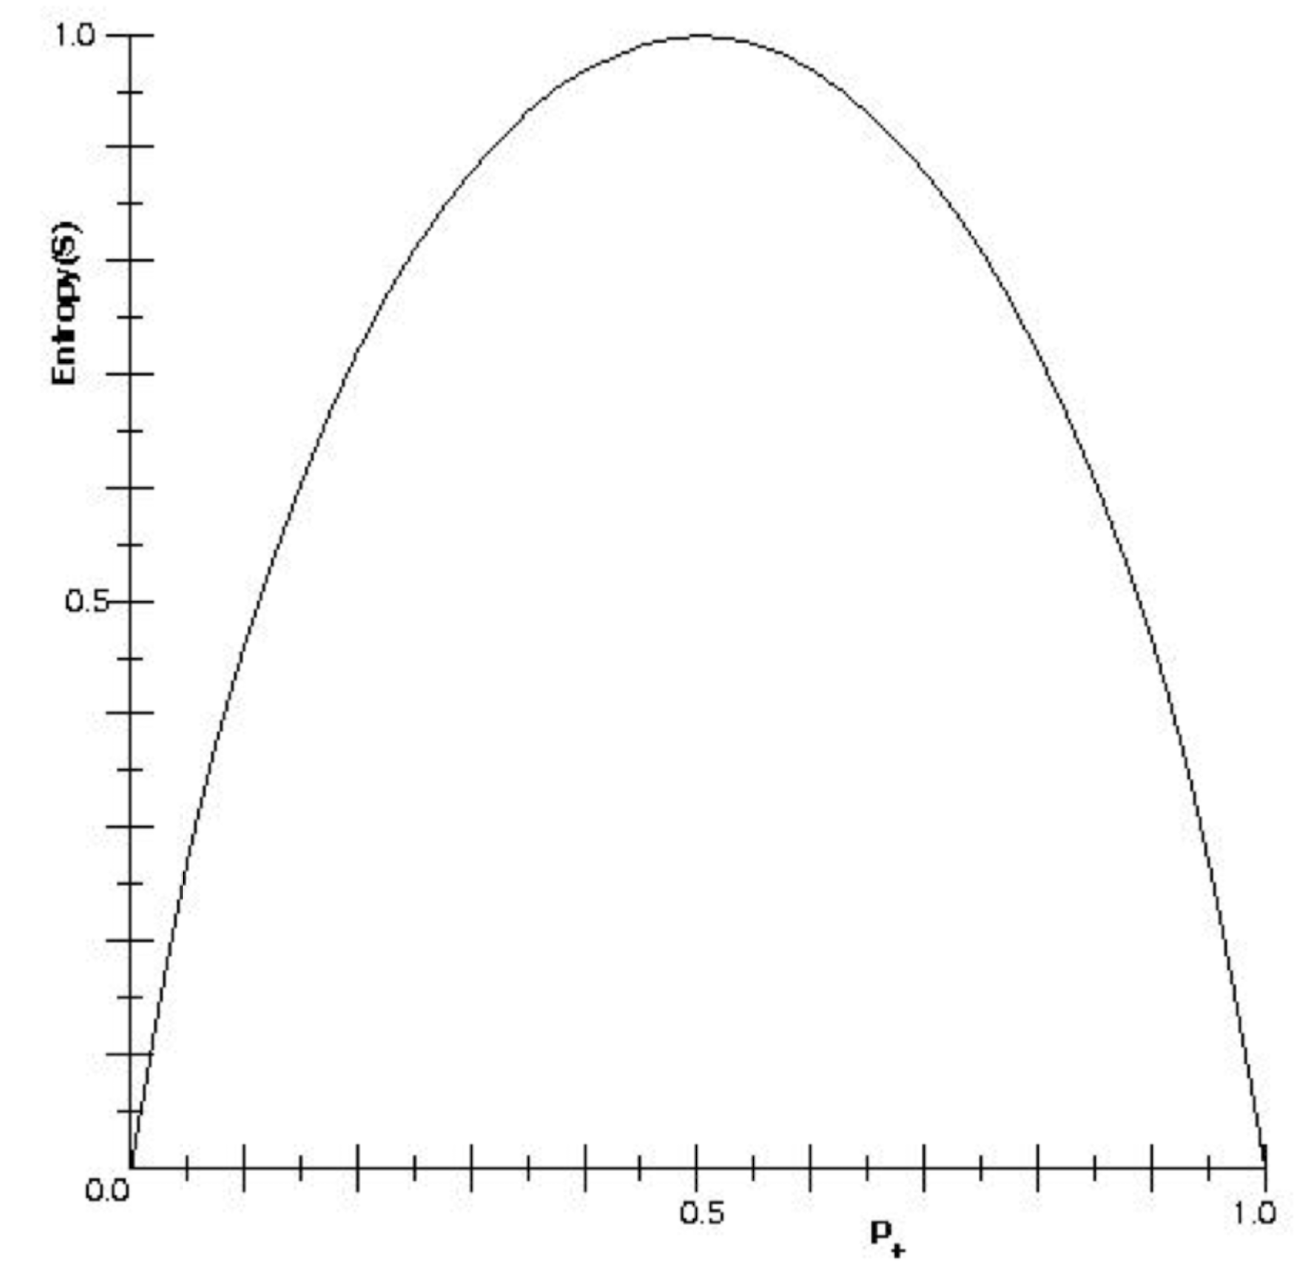
\includegraphics[scale=0.12]{entropy}

    \[I(\frac{p}{p + n}, \frac{n}{p + n}) = \]
    \[- \frac{p}{p + n} \log_{2} \frac{p}{p + n} \]
    \[- \frac{n}{p + n} \log_{2} \frac{n}{p + n}\]

\end{multicols*}

\begin{itemize}
    \item \keyword{Information Gain}{(IG) Reduction in entropy from attribute test} 
    \item Goal: Choose attribute with largest information gain
    \item Intuition: IG = Entropy of this node - Entropy of children nodes
    \item Given chosen attribute $A$ with $v$ distinct values:
\end{itemize}

\[\text{remainder}(A) = \sum_{i = 1}^{v} \frac{p_i + n_i}{p + n} I(\frac{p_i}{p_i + n_i}, \frac{n_i}{p_i + n_i})\]
\[IG(A) = I(\frac{p}{p + n}, \frac{n}{p + n}) - \text{remainder}(A)\]

\begin{itemize}
    \item \keyword{Decision Tree Learning}{Recursively choose attributes with highest IG}
    \item IG is not the only way. Can use whatever objective function that achieves the criteria we want.
\end{itemize}

\subsection{Performance Measurement}

\begin{itemize}
    \item \keyword{Correctness}{Correct if $\hat{y} = y$}
    \item \keyword{Accuracy}{$\frac{1}{m} \sum_{j = 1}^{m} (\hat{y_{j}} = y_{j})$}
\end{itemize}

\begin{multicols*}{2}

    \begin{itemize}
        \item Confusion Matrix:
    \end{itemize}
        
    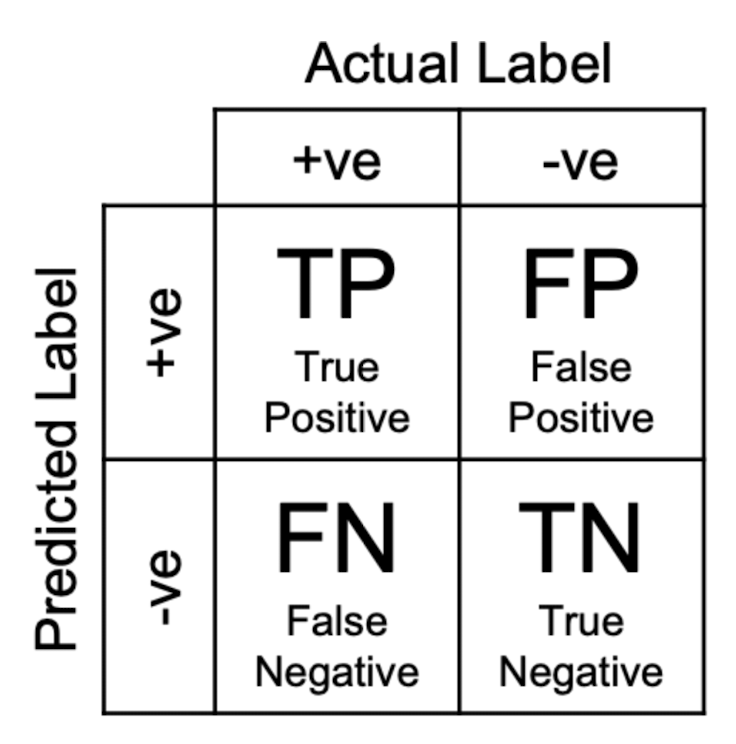
\includegraphics[scale=0.2]{confusion-matrix}

    \begin{itemize}
        \item Accuracy = $\frac{TP + TN}{TP + FN + FP + TN}$
        \item \keyword{Precision}{$\frac{TP}{TP + FP}$} How precise are positive predictions? 
        \item \keyword{Recall}{$\frac{TP}{TP + FN}$} How many actual positives are predicted?
        \item \keyword{F1 Score}{$\frac{2}{1 / P + 1 / R}$} Harmonic mean of precision and recall
    \end{itemize}

\end{multicols*}

\begin{itemize}
    \item Type I Error: FP, Type II Error: FN
    \item FP Rate = $\frac{FP}{FP + TN}$ TP Rate = $\frac{TP}{TP + FN}$
\end{itemize}

\subsection{Pruning}

\begin{itemize}
    \item Motivation: DT overfits to training set, but performs poorly on test set
    \item Occam's Razor: Simple hypothesis preferred
    \item \keyword{Pruning}{Ignores outliers, which reduces overfitting}
    \begin{itemize}
        \item Idea: Go with the majority of T/Fs
        \item E.g. Min-sample, Max-depth
    \end{itemize}
\end{itemize}

  \section{Uncategorized}
  \subsection{$\alpha \beta$-pruning}
  \begin{itemize}
    \item init $\alpha = -\infty, \beta = +\infty$
    \item MAX node: update \& return $\alpha$(max), prune the rest if $\alpha \geq \beta$
    \item MIN: update \& return $\beta$(min),  prune the rest if $\beta \leq \alpha$
  \end{itemize}
  \subsection{Decision Trees}
  \begin{itemize}
    \item if they asking for which attribute chosen first, just compare columns try to match.
    \item the more pure groups the better
    \item Impure large groups affect IG more than Impure small groups.
    \item \textbf{Entropy:}
    \item 0 if certain, 1 if completely uncertain
    \item $H(1,0)/H(0,1) = 0 | H(0.5, 0.5) = 0$
    \item $H(Y) = H(P(y_1)...P(y_k)) = - \sum_{i=1}^{k} P(y_i) \log_2 P(y_i)$
    \item e.g. $-(\frac{1}{6} \log_2 \frac{1}{6} + \frac{1}{3} \log_2 \frac{1}{3} + \frac{1}{2} \log_2 \frac{1}{2})$
    \item \textbf{Specific Conditional Entropy:}
    \item $H(Y \mid X = x) = H(P(y_1 \mid x), \dots, P(y_k \mid x))$
    \item e.g. given x = some value, find the entropy
    \item \textbf{Conditional Entropy:}
    \item $H(Y \mid X) = \sum_{x \in X} [P(X = x)\, H(Y \mid X = x)]$
    \item given specific entropies $H_i$ and probability $p_i$ of each given $x = i$,
    \item Cond Ent = Sum of all $p_i \times H_i $
    \item \textbf{Information Gain:}
    \item $IG(Y, X) = H(Y) - H(Y \mid X)$
    \item \textbf{IG for subnodes:}
    \item IG = Entropy of node - Sum of weighted entropies of groups in the node
    \item \textbf{Remainding Entropy at any point during attribute selection:}
    \item $\sum $ weighted entropies in impure groups
  \end{itemize}

  \section*{Linear \& Logistic Regression Cheatsheet}

  \subsection*{Linear Regression Basics}
  Model: $h_w(x) = w_0 + w_1 x_1$ (bias $w_0$, or use dummy $x_0=1$).\\
  MSE Loss: $L_{MSE}(w) = \frac{1}{2n}\sum_{i=1}^n (h_w(x^{(i)}) - y^{(i)})^2$

  \textbf{Example (6A):} $w=[2,1]^\top$, data: $(0,0),(2,1),(3,2)$\\
  $h(x^{(1)})=2+0=2,\; h(x^{(2)})=2+2=4,\; h(x^{(3)})=2+3=5$\\
  $L_{MSE} = \frac{1}{6}[2^2+3^2+3^2]=\frac{22}{6}=\frac{11}{3}$

  \subsection*{SGD Update (6B)}
  Pick random point $i$. Update:
  \[w \leftarrow w - \alpha \cdot (h_w(x^{(i)}) - y^{(i)}) \begin{bmatrix}1\\x^{(i)}\end{bmatrix}\]
  \textbf{Example:} Random point $i=2$, $\alpha=1/3$.\\
  Residual $= h(x^{(2)})-y^{(2)} = 4-1=3$\\
  $w' = \begin{bmatrix}2\\1\end{bmatrix} - \frac{1}{3}(3)\begin{bmatrix}1\\2\end{bmatrix} = \begin{bmatrix}2\\1\end{bmatrix}-\begin{bmatrix}1\\2\end{bmatrix}=\begin{bmatrix}1\\-1\end{bmatrix}$

  \subsection*{Linear Dependence \& Convexity (6C)}
  If features are linearly dependent (e.g.\ $x_2=3x_1$): loss is convex (not strictly), so GD may converge to \textit{different weights} but \textit{same loss}. Independent features $\Rightarrow$ strictly convex $\Rightarrow$ unique weights. \textbf{Key}: same loss, possibly different weights.
  $A: x \rightarrow h^A, x' \rightarrow h^{A'}$ $B: x \rightarrow h^B, x' \rightarrow h^{B'}$
  training on x (linearly dependent) may produce different weights but same loss. training on x' (linearly independent) will produce same weights same loss

  \subsection*{Feature Scaling for Stability (6D)}
  When features have very different scales (e.g.\ $x_3\sim1000$ vs others $\sim1$):
  \begin{itemize}
    \item \textbf{Standardization}: $(x - \mu)/\sigma$ \quad \checkmark
    \item \textbf{Min-max scaling}: $(x-x_{min})/(x_{max}-x_{min})$ \quad \checkmark
    \item Normal equation fails if features are linearly dependent (non-invertible $X^\top X$)
  \end{itemize}

  \subsection*{Logistic Regression (6E)}
  Use $\sigma(z)=1/(1+e^{-z})$ when predicting \textit{probability}.\\
  Need bias $w_0$ if $P>0.5$ when all $x_i=0$ (since $\sigma(0)=0.5$, need $w_0>0$).\\
  Write as $P(Y|X) = \sigma(w_0+w_1x_1+w_2x_2+w_3x_3)$. Note: $P(Y|X)$ not $P(Y|w)$.

  \subsection*{Normal Equation (6F)}
  $w = (X^\top X)^{-1} X^\top y$\\
  Diagonal matrix inverse: flip each diagonal entry $d_i \to 1/d_i$.\\
  \textbf{Example:} $X=\begin{bmatrix}1&0\\0&2\end{bmatrix}$, $y=\begin{bmatrix}5\\6\end{bmatrix}$\\
  $X^\top X = \begin{bmatrix}1&0\\0&4\end{bmatrix}$, $(X^\top X)^{-1}=\begin{bmatrix}1&0\\0&1/4\end{bmatrix}$\\
  $X^\top y = \begin{bmatrix}5\\12\end{bmatrix}$, $w = \begin{bmatrix}1&0\\0&1/4\end{bmatrix}\begin{bmatrix}5\\12\end{bmatrix}=\begin{bmatrix}5\\3\end{bmatrix}$

  \subsubsection{Inverting 2x2 Matrix}
  $
  \text{For } A = \begin{bmatrix}a&b\\c&d\end{bmatrix}, \quad
  A^{-1} = \frac{1}{ad-bc}\begin{bmatrix}d&-b\\-c&a\end{bmatrix}
  $
  
\end{multicols*}
\end{document}
